% This is the Reed College LaTeX thesis template. Most of the work
% template. Later comments etc. by Ben Salzberg (BTS). Additional
% restructuring and APA support by Jess Youngberg (JY).
% Your comments and suggestions are more than welcome; please email
% them to cus@reed.edu
%
% See http://web.reed.edu/cis/help/latex.html for help. There are a
% great bunch of help pages there, with notes on
% getting started, bibtex, etc. Go there and read it if you're not
% already familiar with LaTeX.
%
% Any line that starts with a percent symbol is a comment.
% They won't show up in the document, and are useful for notes
% to yourself and explaining commands.
% Commenting also removes a line from the document;
% very handy for troubleshooting problems. -BTS

% As far as I know, this follows the requirements laid out in
% the 2002-2003 Senior Handbook. Ask a librarian to check the
% document before binding. -SN

%%
%% Preamble
%%
% \documentclass{<something>} must begin each LaTeX document
\documentclass[12pt,twoside]{reedthesis}
% Packages are extensions to the basic LaTeX functions. Whatever you
% want to typeset, there is probably a package out there for it.
% Chemistry (chemtex), screenplays, you name it.
% Check out CTAN to see: http://www.ctan.org/
%%
\usepackage{graphicx,latexsym}
\usepackage{amsmath}
\usepackage{amssymb,amsthm}
\usepackage{longtable,booktabs,setspace}
\usepackage{chemarr} %% Useful for one reaction arrow, useless if you're not a chem major
\usepackage{rotating}

% Modified by CII
\usepackage[hyphens]{url}
\usepackage{hyperref}
\usepackage{lmodern}

% Added by CII (Thanks, Hadley!)
% Use ref for internal links
\renewcommand{\hyperref}[2][???]{\autoref{#1}}
\def\chapterautorefname{Chapter}
\def\sectionautorefname{Section}
\def\subsectionautorefname{Subsection}

\usepackage{caption}
\captionsetup{width=5in}

% \usepackage{times} % other fonts are available like times, bookman, charter, palatino

\title{Hierarchical Models for Crowdsourced Bicycle Route Ratings}
\author{Will Jones}
% The month and year that you submit your FINAL draft TO THE LIBRARY (May or December)
\date{May 2016}
\division{Mathematics and Natural Sciences}
\advisor{Andrew Bray}
%If you have two advisors for some reason, you can use the following
\altadvisor{}
%%% Remember to use the correct department!
\department{Mathematics}
% if you're writing a thesis in an interdisciplinary major,
% uncomment the line below and change the text as appropriate.
% check the Senior Handbook if unsure.
%\thedivisionof{The Established Interdisciplinary Committee for}
% if you want the approval page to say "Approved for the Committee",
% uncomment the next line
%\approvedforthe{Committee}

% Below added by CII

%%% Copied from knitr
%% maxwidth is the original width if it's less than linewidth
%% otherwise use linewidth (to make sure the graphics do not exceed the margin)
\makeatletter
\def\maxwidth{ %
  \ifdim\Gin@nat@width>\linewidth
    \linewidth
  \else
    \Gin@nat@width
  \fi
}
\makeatother

\renewcommand{\contentsname}{Table of Contents}

\setlength{\parskip}{0pt}


\providecommand{\tightlist}{%
  \setlength{\itemsep}{0pt}\setlength{\parskip}{0pt}}

\Acknowledgements{
I want to thank a few people.
}

\Dedication{
You can have a dedication here if you wish.
}

\Preface{
This is an example of a thesis setup to use the reed thesis document
class.
}

\Abstract{
The preface pretty much says it all.
}

\usepackage{tikz, dsfont}

%%
%% End Preamble
%%
%

\begin{document}

      \maketitle
  
  \frontmatter % this stuff will be roman-numbered
  \pagestyle{empty} % this removes page numbers from the frontmatter

      \begin{acknowledgements}
      I want to thank a few people.
    \end{acknowledgements}
  
      \begin{preface}
      This is an example of a thesis setup to use the reed thesis document
      class.
    \end{preface}
  
  % Add table of abbreviations?

      \hypersetup{linkcolor=black}
    \setcounter{tocdepth}{2}
    \tableofcontents
  
      \listoftables
  
      \listoffigures
  
      \begin{abstract}
      The preface pretty much says it all.
    \end{abstract}
  
      \begin{dedication}
      You can have a dedication here if you wish.
    \end{dedication}
  
  \mainmatter % here the regular arabic numbering starts
  \pagestyle{fancyplain} % turns page numbering back on

  \chapter*{Introduction}\label{introduction}
  \addcontentsline{toc}{chapter}{Introduction}
  
  Knock Software's \emph{Ride Report} app combines a simple
  thumbs-up/thumbs-down rating system with GPS traces of bicycle rides to
  compile a crowdsourced data set of which routes are and are not
  stressful for urban bicyclists.
  
  The app that collects the data is simple: \emph{Ride Report}
  automatically detects when a user start riding their bike, records the
  GPS trace of the route, and then prompts the user at the end of the ride
  to give either a thumbs-up or thumbs-down rating. From this, they were
  able to create a simple ``stress map'' of Portland, OR, which displays
  the average ride rating of rides going through each discretized ride
  segment.
  
  \begin{figure}[h!tbp]
  \centering
  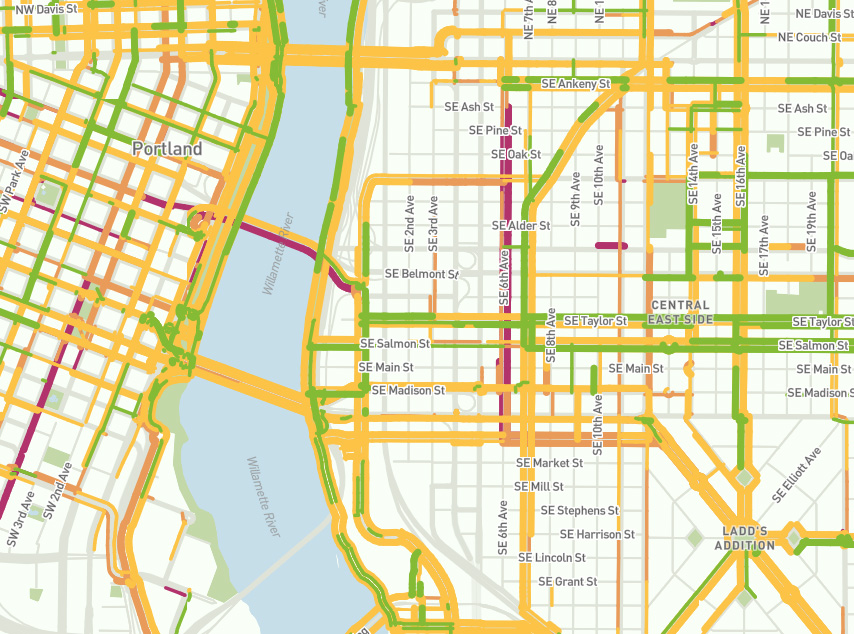
\includegraphics[scale = 1,angle = 0]{figure/stress_map.jpg}
  \caption[Ride Report's Stress Map for Portland. Greener road segments incidate less
  while more red segments indicate more stressful streets. ``Stress'' computed by
  taking the average rating for each segment.]{\normalsize{Ride Report's Stress Map for Portland. Greener road segments incidate less
  while more red segments indicate more stressful streets. ``Stress'' computed by
  taking the average rating for each segment.}}
  \label{fig:stress-map}
  \end{figure}
  
  The app privileges reducing barriers to response to increase sample size
  over ensuring quality and consistent responses. This presents the first
  problem: how can we analyze ratings when riders are likely rating rides
  inconsistently?
  
  At the same time, we have another challenge. We have ratings associated
  with routes, but we would like to know the effect of particular road
  segments, for both inference (what effect does this road segment have on
  the rating?) and prediction (given a route, what do we expect the rating
  to be?) purposes.
  
  Finally, there are interesting issues with missing data. First, the
  sample of rides we have are biased towards routes that riders percieve
  as better. Second, a significant portion of the rides are missing a
  response, and non response is unlikely to be independent of the
  response. The good news is that we have all the predictors for every
  ride, enabling us to build a model that is able to leverage the data
  with missing responses rather than listing the missing data as a
  liability.
  
  \section{Accounting for Rider Rating
  Variance}\label{accounting-for-rider-rating-variance}
  
  For ratings we are interested in modeling variance between riders (as we
  might expect riders to have different rating patterns than their peers)
  and within riders (as riders may not rate the same route and conditions
  the same every time). To model this, we propose using multilevel
  regression, with random effects from each rider. This approach has been
  used in similar situations, in one case to model sexual
  attraction\footnote{Mackaronis, Strassberg, Cundiff, \& Cann (2013)}.
  
  In a multilevel model, we fit a regression where the intercept term
  varies by group but comes from a common distribution. For example, if we
  let \(r_i\) be the rating of the \(i\)th ride, \(X_i\) be the ride-level
  variables, then we can fit a regression:
  
  \[\mathbb{P}(r_i = 1) = \text{logit}^{-1}
  \left( \alpha_{j[i]} +  X_i \beta \right) ,\] where \(\alpha_j\) is an
  intercept specific to rider \(j\). In addition, the rider intercepts
  come from a common distribution,
  \[\alpha_j \sim N (\mu_\alpha, \sigma^2_\alpha),\]
  
  where \(\mu_\alpha\) is the mean of all the \(\alpha_j\)s.
  
  Using varying intercepts will allow our model to exhibit the property of
  varying rates of riders giving stressful ratings. This can be extended
  to model differences in how riders respond to different kinds of road
  conditions using varying slope models. We explore multilevel model
  further in Section \autoref{h-models} and multilevel models for riders
  in Section \autoref{add-riders}.
  
  \section{Addressing Road Segments as a
  Level}\label{addressing-road-segments-as-a-level}
  
  We examine multiple approaches to modeling road segments. In the first,
  we regard add regression term for the route, that is a weighted sum of
  terms for each road segment in the route, weighted by the lengths of the
  segments. The terms for the
  
  the contribution of the route to be a weighted sum of the contributions
  of road segments in the route, weighted by the lengths of the segments.
  
  \section{Approaching Missing Data at Multiple
  Levels}\label{approaching-missing-data-at-multiple-levels}
  
  This data set contains missing data at two levels.
  
  First, there are many routes without any ratings. The routes taken by
  riders are not a random sample of routes, but are often already chosen
  by the rider as the least stressful ride. As we might expect because of
  this bias, only a small proportion of rides are rated as ``stressful.''
  
  One solution we explore to this problem is adding a segment popularity
  parameter as a segment-level predictor.
  
  Second, not every ride is given a rating. We do have the route they
  chose, and all associated covariates, but the response variable, rating
  is missing. As we will discuss in chapter \autoref{missing-data}, the
  pattern of non-response is unlikely to be unbiased.
  
  To address the second problem, we first build a separate probability
  model that predicts non response, and then integrate that model into our
  main model.
  
  \chapter{Data Sources}\label{rmd-basics}
  
  Here is a brief introduction into using \emph{R Markdown}.
  \emph{Markdown} is a simple formatting syntax for authoring HTML, PDF,
  and MS Word documents. \emph{R Markdown} provides the flexibility of
  \emph{Markdown} with the implementation of \textbf{R} input and output.
  For more details on using \emph{R Markdown} see
  \url{http://rmarkdown.rstudio.com}.
  
  Be careful with your spacing in \emph{Markdown} documents. While
  whitespace largely is ignored, it does at times give \emph{Markdown}
  signals as to how to proceed. As a habit, try to keep everything left
  aligned whenever possible, especially as you type a new paragraph. In
  other words, there is no need to indent basic text in the Rmd document
  (in fact, it might cause your text to do funny things if you do).
  
  \section{Ride Report}\label{ride-report}
  
  It's easy to create a list. It can be unordered like
  
  \begin{itemize}
  \tightlist
  \item
    Item 1
  \item
    Item 2
  \end{itemize}
  
  or it can be ordered like
  
  \begin{enumerate}
  \def\labelenumi{\arabic{enumi}.}
  \tightlist
  \item
    Item 1
  \item
    Item 2
  \end{enumerate}
  
  Notice that I intentionally mislabeled Item 2 as number 4.
  \emph{Markdown} automatically figures this out! You can put any numbers
  in the list and it will create the list. Check it out below.
  
  To create a sublist, just indent the values a bit (at least four spaces
  or a tab). (Here's one case where indentation is key!)
  
  \begin{enumerate}
  \def\labelenumi{\arabic{enumi}.}
  \tightlist
  \item
    Item 1
  \item
    Item 2
  \item
    Item 3
  
    \begin{itemize}
    \tightlist
    \item
      Item 3a
    \item
      Item 3b
    \end{itemize}
  \end{enumerate}
  
  \section{Weather Data}\label{weather-data}
  
  Make sure to add white space between lines if you'd like to start a new
  paragraph. Look at what happens below in the outputted document if you
  don't:
  
  Here is the first sentence. Here is another sentence. Here is the last
  sentence to end the paragraph. This should be a new paragraph.
  
  \emph{Now for the correct way:}
  
  Here is the first sentence. Here is another sentence. Here is the last
  sentence to end the paragraph.
  
  This should be a new paragraph.
  
  \section{Road Data}\label{road-data}
  
  When you click the \textbf{Knit} button above a document will be
  generated that includes both content as well as the output of any
  embedded \textbf{R} code chunks within the document. You can embed an
  \textbf{R} code chunk like this (\texttt{cars} is a built-in \textbf{R}
  dataset):
  
  \chapter{Data Transformation}\label{data-trans}
  
  \section{Working in Road Networks}\label{working-in-road-networks}
  
  \section{Using Nearest Neighbor Search for Map Matching
  Data}\label{using-nearest-neighbor-search-for-map-matching-data}
  
  \section{Missing Data}\label{missing-data}
  
  \chapter{Methods}\label{methods}
  
  As an undergraduate thesis, a lot of research into methodology was done.
  Here I go through some of the essential methodology, while establishing
  the notation I will use for the rest of this paper.
  
  \section{Logistic Regression}\label{logistic-regression}
  
  With logistic regression, we seek to fit a model where the response
  variable is binary. We might consider the response variable, \(Y\), a
  Bernoulli random variable,
  
  \[Y = \text{Bernoulli}(p),\]
  
  where \(p\) is the probability that an observation \(y_i = 1,\) for any
  \(i\). (As a binary variable, the support of \(Y\) is \(\{0,1\}\), so
  \(y_i = 0\) otherwise.) Thus, in predicting and making inference about a
  Bernoulli variable, we are concerned with \(p\) and how it varies with
  respect to other quantities.
  
  Logistic regression is, as we will see, one form of regression
  generalized from linear regression.
  
  Linear regression is the first form of regression most people learn:
  find the line
  
  \[y_i = \beta_0 + \beta_1 x_1 + \ldots + \beta_j x_j + \epsilon,\]
  
  based on data with response variable \(y_i\) and \(j\) predictor
  variables \(x_i\), coefficients \(\beta_0, \ldots, \beta_j\), and error
  term \(\epsilon \sim N(0, \sigma^2)\). We can equivalently write,
  
  \[Y \sim N(\beta_0 + \beta_1 x_1 + \ldots + \beta_j x_j, \sigma^2).\]
  
  Generalized linear regression uses a ``link function,'' \(g\), to modify
  the regression:
  
  \[g(y_i) = \beta_0 + \beta_1 x_1 + \ldots + \beta_j x_j + \epsilon.\]
  
  Logistic regression is a form of generalized regression where the `link'
  function is the logit function, \(\text{logit}:[0,1] \to \mathbb{R}\):
  
  \[ \text{logit} (p) = \log \left(\frac{p}{1-p}\right), \]
  
  also known as the log-odds, odds being \(p/1-p\) for any probability
  \(p\). So we can model this as a Bernoulli random variable where the
  probability of a 1 is:
  
  \[\mathbb{P} (y_i = 1) = \text{logit}^{-1} (\beta_0 + \beta_1 x_1 + \ldots + \beta_j x_j).\]
  
  Notice that the inverse logit function maps values from \(\mathbb{R}\)
  to \([0,1]\). The function provides a convenient way to map linear
  combinations of other variables onto values that are valid
  probabilities. Other such functions exist and are also used for
  regression of binary variables, such as the probit function.
  
  \begin{center}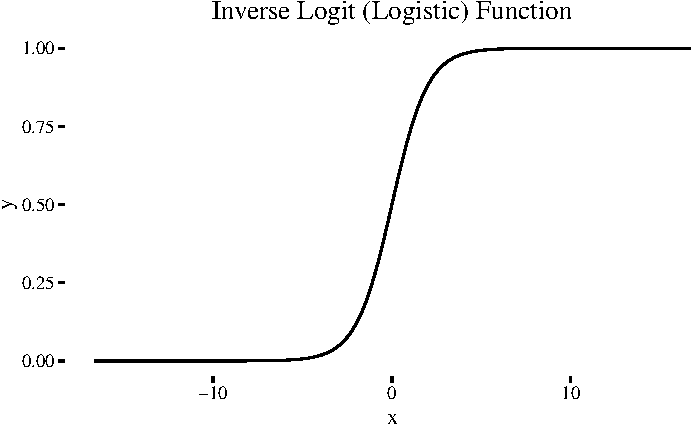
\includegraphics{thesis_files/figure-latex/unnamed-chunk-2-1} \end{center}
  
  Logistic regression is sometimes presented as a classification model
  
  \section{Hierarchical Models and Mixed Effects Models}\label{h-models}
  
  Many data sets contain nested structures when viewed in some way. For
  example, a data set of student test scores may contain information about
  the schools and districts they are in. Or a dataset of soil samples may
  have multiple samples from each of a set of different sites. In the
  dataset we examine, rides can be grouped by rider.
  
  Mutlilevel models allow us to address these kinds of relationships in
  regression models. They provide a number of computational advantages, as
  we shall describe later.
  
  \subsection{Description and Notation}\label{description-and-notation}
  
  These models of course work for other forms of regression, but we will
  focus on logistic regression, as it is the method we use in this paper.
  We will be using notation adapted from Gelman's description of
  multilevel models. Consider a data set composed of
  
  \begin{itemize}
  \tightlist
  \item
    \(i\) observations of a binary response variable \(y_i\),
  \item
    \(m\) observation level predictors \(X_i = x_i^1, \ldots, x_i^m\),
  \item
    \(j\) groups in which the observations are split into,
  \item
    \(l\) group level predictors
    \(U_{j[i]} = u_{j[i]}^1, \ldots, u_{j[i]}^l\), where \(j[i]\) is the
    group of the \(i\)th observation,.
  \end{itemize}
  
  We could fit a model where the intercept varies by group:
  
  \[\mathbb{P} (y_i = 1) = \text{logit}^{-1}
  (\alpha_{j[i]} + X_i \beta),\]
  \[\alpha_{j[i]} \sim N(\gamma_0 + U_{j[i]} \gamma, \sigma_{\alpha}^2),\]
  
  where \(\alpha_{j[i]}\) is the intercept for the \(j\)th group,
  \(\beta\) are the coefficients for the observation-level predictors,
  \(\gamma_0\) are the group-level intercepts, and \(\gamma\) are the
  coefficients for the group-level predictors. We could also imagine a
  similar model where there are no group level predictors, such that we
  simply have different intercepts for each group,
  \[\alpha_{j[i]} \sim N(\gamma_0, \sigma_{\alpha}^2),\]
  
  We can also consider a model that has slopes varying by group. For
  simplicity, let's consider just one observation level predictor,
  \(x_i\), that will have varying slopes \(\beta_{j[i]}\) as well as one
  group level predictor. We could specify the model as,
  
  \[\mathbb{P} (y_i = 1) = \text{logit}^{-1}
  (\alpha_{j[i]} + \beta_{j[i]} x_i),\]
  
  \[
  \left(
  \begin{array}{c}
  \alpha_{j}\\
  \beta_{j}
  \end{array}
  \right) =
  N \left(
  \left(
  \begin{array}{c}
  \gamma_0^\alpha + \gamma_1^\alpha u_j\\
  \gamma_0^\beta + \gamma_1^\beta u_j
  \end{array}
  \right),
  \left(
  \begin{array}{cc}
  \sigma^2_\alpha & \rho \sigma_\alpha \sigma_\beta\\
  \rho \sigma_\alpha \sigma_\beta & \sigma^2_\beta
  \end{array}
  \right)
  \right).
  \]
  
  \subsection{Examples and Advantages}\label{examples-and-advantages}
  
  Gelman puts forward a framework for thinking about multilevel models as
  a comprimise between no-pooling and complete pooling. For example, for
  the school example, one could fit a classical regression ignoring the
  schoolwide data, with students as the level of observation. (That would
  be ``no pooling''.) Alternatively, one could fit a separate regression
  for each school.
  
  \section{Tools for evaluating models}\label{tools-for-evaluating-models}
  
  There are a couple ways we wish to evaluate our models. Most of the
  time, we will compare them to some other model.
  
  Predictive accuracy will be one aspect of our model we will want to
  evaluate. We will use cross-validation to evaluate accuracy, usually
  with \(K\)-fold cross-validation. Statistics such as misclassification
  rate, false-positive rate, and true-negative rate can be calculated for
  each validation. For a more comprehensive look at predictive accuracy,
  we use the separation plot.
  
  \subsection{The Separation Plot}\label{the-separation-plot}
  
  The separation plot, created by \_\_\_\_ in their paper \_\_\_\_, is
  designed to show how well a logistic regression model can distinguish
  between high and low probability events.
  
  Creating a separation plot first requires a model fit to training data
  and testing data to evaluate predictive accuracy on. From the testing
  data, we need a vector \(Y\) of observed binary response data and a
  vector \(\hat{Y}\) of predicted probabilities of a 1 for each
  observation, predicted using our model fitted to training data.
  
  We plot the data \((Y, \hat{Y}\) as a sequence of vertical strips,
  colored according to observed outcome, \(Y\), and ordered from low to
  high probability based on \(\hat{Y}\). A curve is superimposed upon the
  stripes showing the \(\hat{Y}\) as a line graph. And finally, a small
  triangle is placed indicated the point at which the two colors of lines
  would meet if all observations \(Y = 0\) were placed to the left of all
  the \(Y=1\) observations; in other words showing where the boundary
  would be if the two classes were perfectly separated by the model.
  
  \begin{center}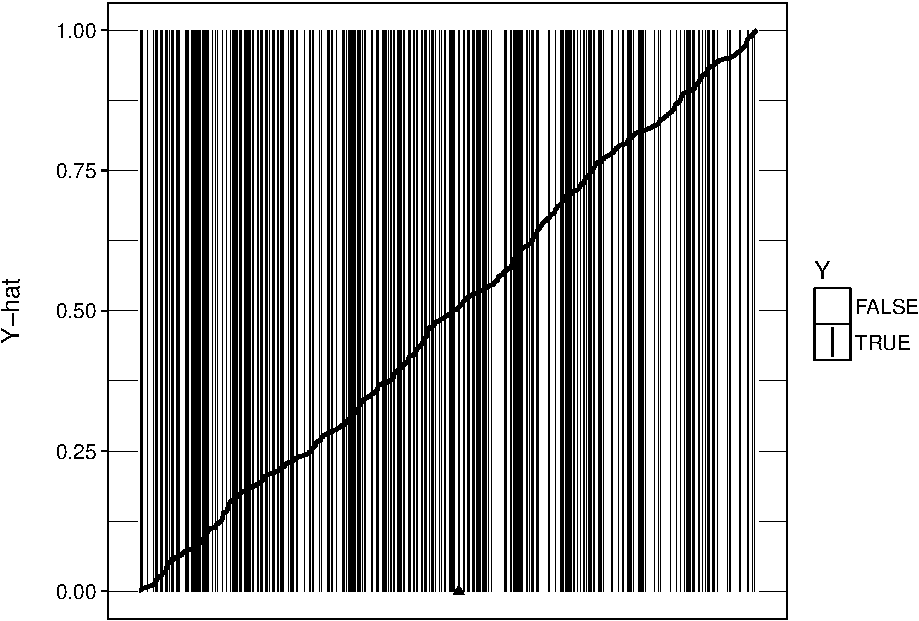
\includegraphics{thesis_files/figure-latex/unnamed-chunk-3-1} \end{center}
  
  \begin{center}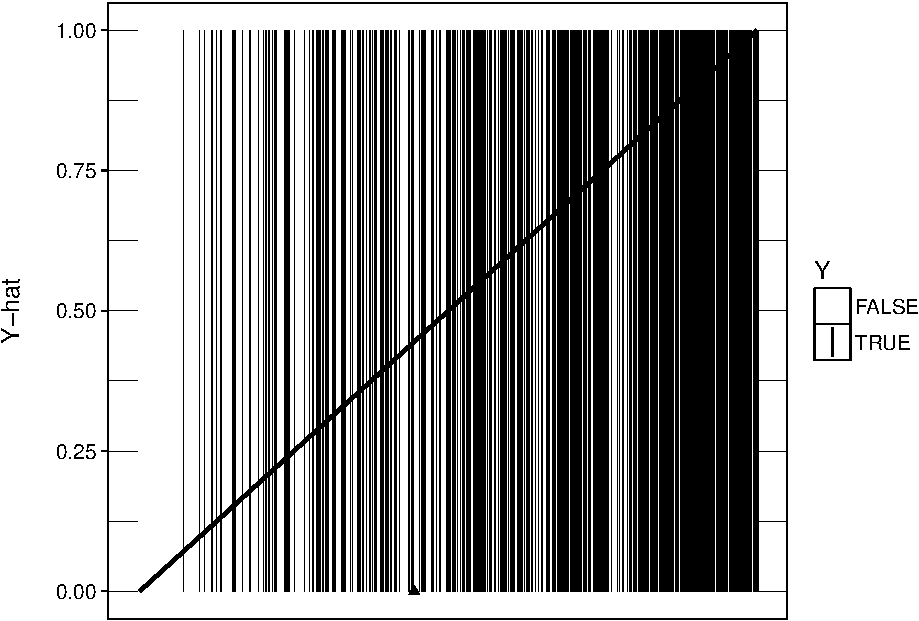
\includegraphics{thesis_files/figure-latex/unnamed-chunk-3-2} \end{center}
  
  \begin{center}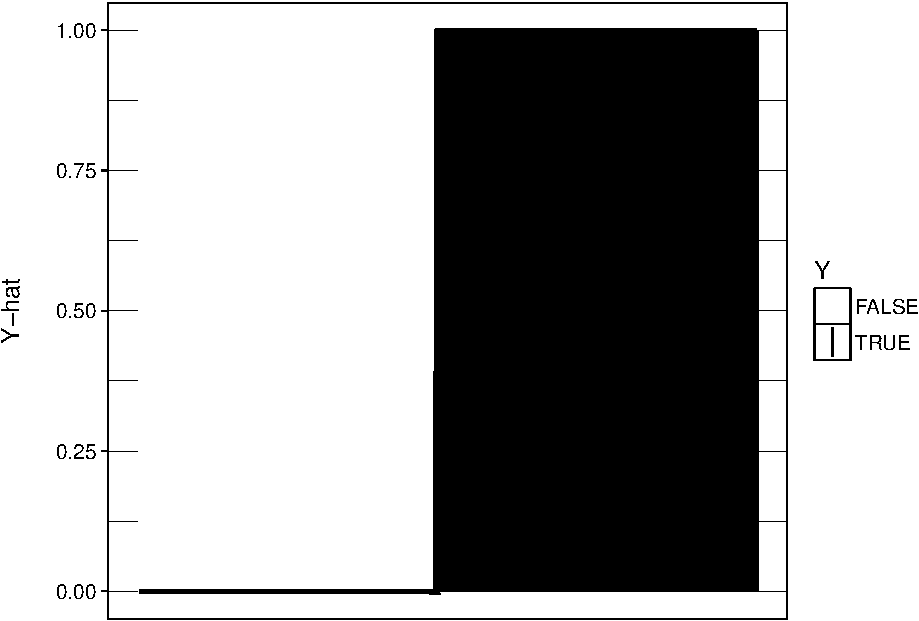
\includegraphics{thesis_files/figure-latex/unnamed-chunk-3-3} \end{center}
  
  Above we have examples of three separation plots. The first plot shows
  what it looks like when \(Y\) and \(\hat{Y}\) are uncorrelated. The
  second plot
  
  \chapter{Model 1: Rides and Riders}\label{model-1-rides-and-riders}
  
  We start out model simply and then building up. The first problem to
  approach is handling rider variance. This sections describes how we do
  that using a random effects terms and demonstrates the improvement in
  the models fit and predictive accuracy over more classical models.
  
  \section{Choosing Ride-Level
  Parameters}\label{choosing-ride-level-parameters}
  
  \subsection{Weather}\label{weather}
  
  \subsection{Traffic}\label{traffic}
  
  We would like to have some model for the effect of traffic. We don't
  have actual traffic data, but we do know that there are fluxuations in
  how riders rate rides based on time of day, with somewhat higher rates
  during the morning and evening. The simplist way to model this might be
  a rush hour indicator:
  
  \[ x_i^{\text{rush.hour}} = 
  \mathds{1} [x_i^{\text{time}} \text{during rush hour}],
  \]
  
  where rush hour is defined as between 7 a.m. and 9 a.m. and 5 p.m. and 7
  p.m. on weekdays. However this maybe a little too naive. We might also
  want to simply have a term that absorbed all time of day difference in
  ratings.
  
  We might consider adding a term that is a sinusoidal function with a
  period of one day. We would be interested in fitting a term,
  
  \[A \sin (T x^{\text{time}} + \phi),\]
  
  where \(\beta\) and \(\phi\) are coefficients estimated and
  \(T = 2 \pi / d,\) where \(d\) is the period of one day
  (\(8.64 \times 10^7\) milliseconds.) This form isn't easy to estimate,
  but we can transform this expression into the sum of two trignometric
  functions:
  
  \begin{align*}
  A \sin (T x + \phi) &= 
  A \left( \sin (T x) \cos (\phi) + \cos (T x) \sin (\phi) \right)\\
  &= (A + \cos (\phi)) \sin (T x) + \sin (\phi) \cos (T x)\\
  &= \beta_1 \sin (T x) + \beta_2 \cos (T x),
  \end{align*}
  
  where \(\beta_1 = A + \cos (\phi)\) and \(\beta_2 = \sin (\phi).\) This
  term won't model just traffic; it will probably absorb all effects that
  are cyclical over the day.
  
  \section{Adding Random Effects from Riders}\label{add-riders}
  
  \section{Evaluating the Ride-Level
  Models}\label{evaluating-the-ride-level-models}
  
  \chapter{Model 2: Regression Terms for Road
  Segments}\label{model-2-regression-terms-for-road-segments}
  
  Now we have the task of incorporating our knowledge of riders' routes
  into our regression. Our approach here will be to consider routes as
  sequences of discrete road segments, each of which have known
  properties. This is convenient because we have such data about roads
  that give us bike lanes, road size, etc. It is even possible for us to
  calculate popularity of particular segments easily.
  
  Assume we have \(K\) total road segments in our road network and for
  each ride we have \(\Omega_i \subseteq \{1, \ldots, K\}\), the set of
  road segments that are in the route of ride \(i\). Let \(l_k\) be the
  length of the \(k\)th segment and define the length of ride \(i\) to be:
  
  \[ L_i = \sum_{k \in \Omega_i} l_k.\]
  
  For the \(k\)th road segment, define the m-dimensional vector
  \(W_k = W_k^1, W_k^2, \ldots, W_k^m\) road segment-level predictors.
  Then we shall define the term in our regression for the route of ride
  \(i\) as
  
  \[ R_i = \frac{1}{L_i} \sum_{k \in \Omega_i} l_k W_k \beta^{\text{road}},\]
  
  Where \(\beta^{\text{road}}\) is a vector of coefficients for the road
  segment level predictors. When actually computing this value, it may be
  convenient to factor out the \(\beta^{\text{road}}\)
  
  \section{Choosing Segment-Level
  Parameters}\label{choosing-segment-level-parameters}
  
  \section{Evaluating Segment-Level
  Models}\label{evaluating-segment-level-models}
  
  \chapter{Model 3: A Spatial Model}\label{model-3-a-spatial-model}
  
  \chapter{Comparative Evaluation}\label{comparative-evaluation}
  
  \chapter*{Conclusion}\label{conclusion}
  \addcontentsline{toc}{chapter}{Conclusion}
  
  \setcounter{chapter}{4} \setcounter{section}{0}
  
  If we don't want Conclusion to have a chapter number next to it, we can
  add the \texttt{\{.unnumbered\}} attribute. This has an unintended
  consequence of the sections being labeled as 3.6 for example though
  instead of 4.1. The \LaTeX~commands immediately following the Conclusion
  declaration get things back on track.
  
  \subsubsection{More info}\label{more-info}
  
  And here's some other random info: the first paragraph after a chapter
  title or section head \emph{shouldn't be} indented, because indents are
  to tell the reader that you're starting a new paragraph. Since that's
  obvious after a chapter or section title, proper typesetting doesn't add
  an indent there.
  
  \backmatter
  
  \chapter{References}\label{references}
  
  \noindent
  
  \setlength{\parindent}{-0.20in} \setlength{\leftskip}{0.20in}
  \setlength{\parskip}{8pt}
  
  \hypertarget{refs}{}
  \hypertarget{ref-cressie2011}{}
  Cressie, N., \& Wikle, C. K. (2011). \emph{Statistics for
  spatio-temporal data}. John Wiley \& Sons.
  
  \hypertarget{ref-gelman}{}
  Gelman, A., \& Hill, J. (2006). \emph{Data analysis using regression and
  multilevel/Hierarchical models}. The Edinburgh Building, Cambridge CB2
  8RU, UK: Cambridge University Press, New York.
  
  \hypertarget{ref-mackaronis2013}{}
  Mackaronis, J. E., Strassberg, D. S., Cundiff, J. M., \& Cann, D. J.
  (2013). Beholder and beheld: A multilevel model of perceived sexual
  appeal. \emph{Archives of Sexual Behavior}.


  % Index?

\end{document}

